\chapter{Introduction to Network
Automation}\label{introduction-to-network-automation}

\section{Why Network Automation}\label{why-network-automation}

\begin{itemize}
\tightlist
\item
  Previous versions of the CCNA focused on the traditional model of
  managing / controlling networks
\item
  The current version focuses on the traditional model as well, but CCNA
  candidates are expected to have a basic understanding of various
  topics related to network automation
\item
  In the traditional model, engineers manage devices one at a time by
  connecting to their CLI via SSH
\end{itemize}

\section{Downsides of Configuring Devices
One-by-One}\label{downsides-of-configuring-devices-one-by-one}

\begin{itemize}
\tightlist
\item
  Typos and other small mistakes are common
\item
  It is time-consuming and very inefficient in large-scale networks
\item
  It is difficult to ensure that all devices ADHERE to the
  organization's STANDARD CONFIGURATION
\end{itemize}

\section{Benefits of Network
Automation}\label{benefits-of-network-automation}

\begin{itemize}
\tightlist
\item
  Human Error (Typos, etc) is reduced
\item
  Networks become much more scalable and implemented in a fraction of
  the time

  \begin{itemize}
  \tightlist
  \item
    New deployments
  \item
    Network-wide changes
  \item
    Troubleshooting
  \end{itemize}
\item
  Network-wide policy compliance can be assured

  \begin{itemize}
  \tightlist
  \item
    Standard configurations
  \item
    Software versioning
  \end{itemize}
\item
  The improved efficiency of network operations reduces the OP-EX
  (operating expenses) of the network. Each task requires fewer
  man-hours
\end{itemize}

\begin{lstlisting}
There are various tools / methods that can be used to automate tasks in the network

- SDN (Software-Defined Networking)
- Ansible
- Puppet
- Python scripts
- etc...
\end{lstlisting}

LOGICAL ``PLANES'' OF NETWORK FUNCTIONS

\textbf{What does a ROUTER do?}

\begin{itemize}
\tightlist
\item
  It forwards messages between networks by examining information in the
  Layer 3 header
\item
  It uses a routing protocol like OSPF to share route information with
  other routers and build a routing table
\item
  It uses ARP to build an ARP table, mapping IP Addresses to MAC
  Addresses
\item
  It uses Syslog to keep logs of events that occur
\item
  and MUCH more\ldots{}
\end{itemize}

\textbf{What does a SWITCH do?}

\begin{itemize}
\tightlist
\item
  It forwards messages within a LAN by examining information in the
  Layer 2 header
\item
  It uses STP to ensure there are no Layer 2 loops in the network
\item
  It builds a MAC address table by examining the Source MAC address of
  frames
\item
  It uses Syslog to keep logs of events that occur
\item
  It allows a user to connect to it via SSH and manage it
\end{itemize}

The various functions of network devices can be logically divided up
(categorized) into \emph{PLANES}

\begin{lstlisting}
- DATA PLANE
- CONTROL PLANE
- MANAGEMENT PLANE
\end{lstlisting}

\begin{itemize}
\tightlist
\item
  The operations of the MANAGEMENT PLANE and the CONTROL PLANE are
  usually managed by the CPU
\item
  However, this is not desirable for DATA PLANE operations because CPU
  processing is slow (relatively speaking)
\item
  Instead, a specialized hardware ASIC (Application-Specific Integrated
  Circuit) is used.

  \begin{itemize}
  \tightlist
  \item
    ASICs are chips built for a specific purpose
  \end{itemize}
\item
  Using a SWITCH, as an example:

  \begin{itemize}
  \tightlist
  \item
    When a FRAME is received, the ASIC (not the CPU) is responsible for
    the switching logic
  \item
    The MAC Address table is stored in a kind of memory called TCAM
    (Ternary Content-Addressable Memory)

    \begin{itemize}
    \tightlist
    \item
      Another common name for the MAC Address table is CAM TABLE
    \end{itemize}
  \item
    The ASIC feeds the DESTINATION MAC address of the FRAME into the
    TCAM which returns the matching MAC Address table entry
  \item
    The FRAME is then forwarded out of the appropriate DEVICE
  \end{itemize}
\item
  Modern ROUTERS also use a similar hardware DATA PLANE: An ASIC
  designed for forwarding logic, and tables store in TCAM
\end{itemize}

\section{A Simple Summary}\label{a-simple-summary}

\begin{quote}
\begin{itemize}
\tightlist
\item
  When a DEVICE receives CONTROL / MANAGEMENT traffic (destined for
  itself), it will be processed in the CPU
\item
  When a DEVICE receives DATA traffic which should pass through the
  DEVICE, it is processed by the ASIC for maximum speed
\end{itemize}
\end{quote}

\section{Data Plane}\label{data-plane}

\begin{itemize}
\tightlist
\item
  All tasks involved in forwarding USER DATA / TRAFFIC from one
  INTERFACE to another are part of the DATA PLANE
\item
  A ROUTER receives a message, looks for the most specific matching
  ROUTER in its ROUTING TABLE, and forwards it out of the appropriate
  INTERFACE to the next hop

  \begin{itemize}
  \tightlist
  \item
    It also de-encapsulates the original LAYER 2 header, and
    re-encapsulates with a new header destined for the next hop's MAC
    address
  \end{itemize}
\item
  A SWITCH receives a message, looks at the DESTINATION MAC Address, and
  forwards it out of the appropriate INTERFACE (or FLOODS it)

  \begin{itemize}
  \tightlist
  \item
    This includes functions like adding / removing 802.1q VLAN tags
  \end{itemize}
\item
  NAT (changing the SRC / DST addresses before forwarding) is part of
  the DATA PLANE
\item
  Deciding to forward / discard messages due to ACL's, port-security,
  etc. is part of the DATA PLANE
\item
  The DATA PLANE is also called the `FORWARDING PLANE'
\end{itemize}

\begin{figure}
\centering
\pandocbounded{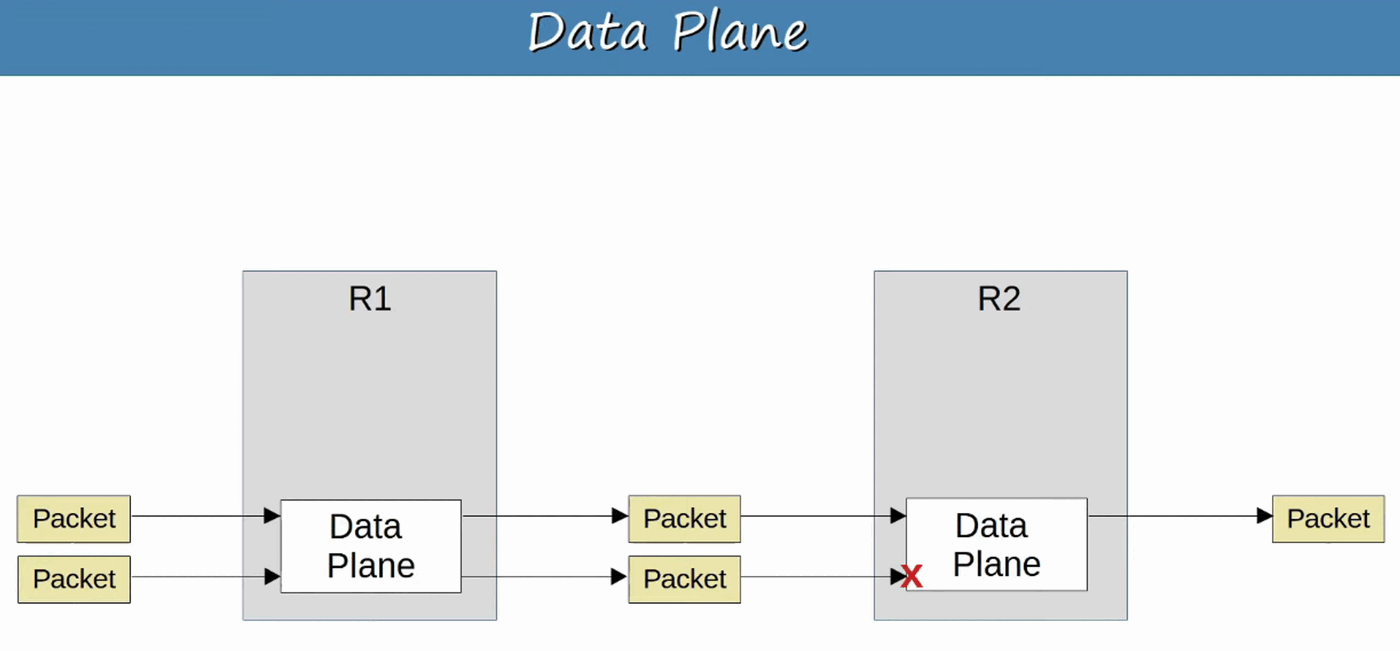
\includegraphics[keepaspectratio,alt={image}]{images/62-introduction-to-network-automation/img-001.png}}
\end{figure}

\section{Control Plane}\label{control-plane}

\begin{itemize}
\item
  How does a DEVICE's DATA PLANE make its forwarding decisions?

  \begin{itemize}
  \tightlist
  \item
    ROUTING TABLE
  \item
    MAC ADDRESS table
  \item
    ARP table
  \item
    STP
  \item
    etc\ldots{}
  \end{itemize}
\item
  Functions that build THESE tables (and other functions that influence
  the DATA PLANE) are part of the CONTROL PLANE
\item
  The CONTROL PLANE \emph{controls} what the DATA PLANE does, for
  example by building the ROUTER's ROUTING TABLE
\item
  The CONTROL PLANE performs \emph{overhead} work

  \begin{itemize}
  \tightlist
  \item
    OSPF itself doesn't forward user data packets, but it informs the
    DATA PLANE about HOW packets should be forwarded
  \item
    STP itself isn't directly involved in the process of forwarding
    FRAMES, but it informs the DATA PLANE about which INTERFACES should
    and shouldn't be used to forward FRAMES
  \item
    ARP messages aren't user data but they are used to build an ARP
    TABLE which is used in the process of forwarding data
  \end{itemize}
\end{itemize}

\begin{figure}
\centering
\pandocbounded{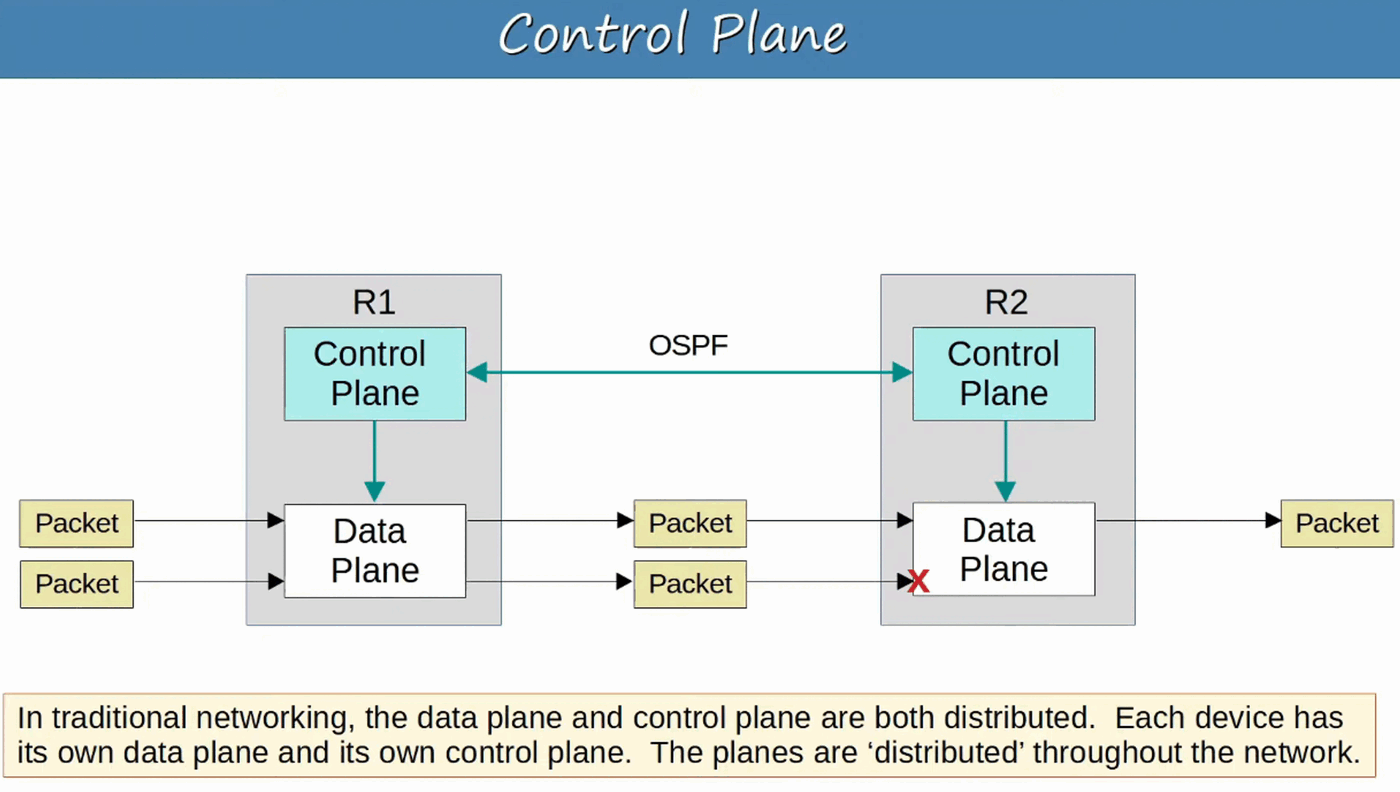
\includegraphics[keepaspectratio,alt={image}]{images/62-introduction-to-network-automation/img-002.png}}
\end{figure}

\section{Management Plane}\label{management-plane}

\begin{itemize}
\tightlist
\item
  Like the CONTROL PLANE, the MANAGEMENT PLANE performs overhead work

  \begin{itemize}
  \tightlist
  \item
    However, the MANAGEMENT PLANE doesn't directly affect the forwarding
    of messages in the DATA PLANE
  \end{itemize}
\item
  The MANAGMENT PLANE consists of PROTOCOLS that are used to manage
  devices

  \begin{itemize}
  \tightlist
  \item
    SSH / TELNET : Used to connect to the CLI of a DEVICE to configure /
    manage it
  \item
    SYSLOG : Used to keep logs of events that occur on the device
  \item
    SNMP : Used to monitor the operations of the device
  \item
    NTP : Used to maintain accurate time on the device
  \end{itemize}
\end{itemize}

\begin{figure}
\centering
\pandocbounded{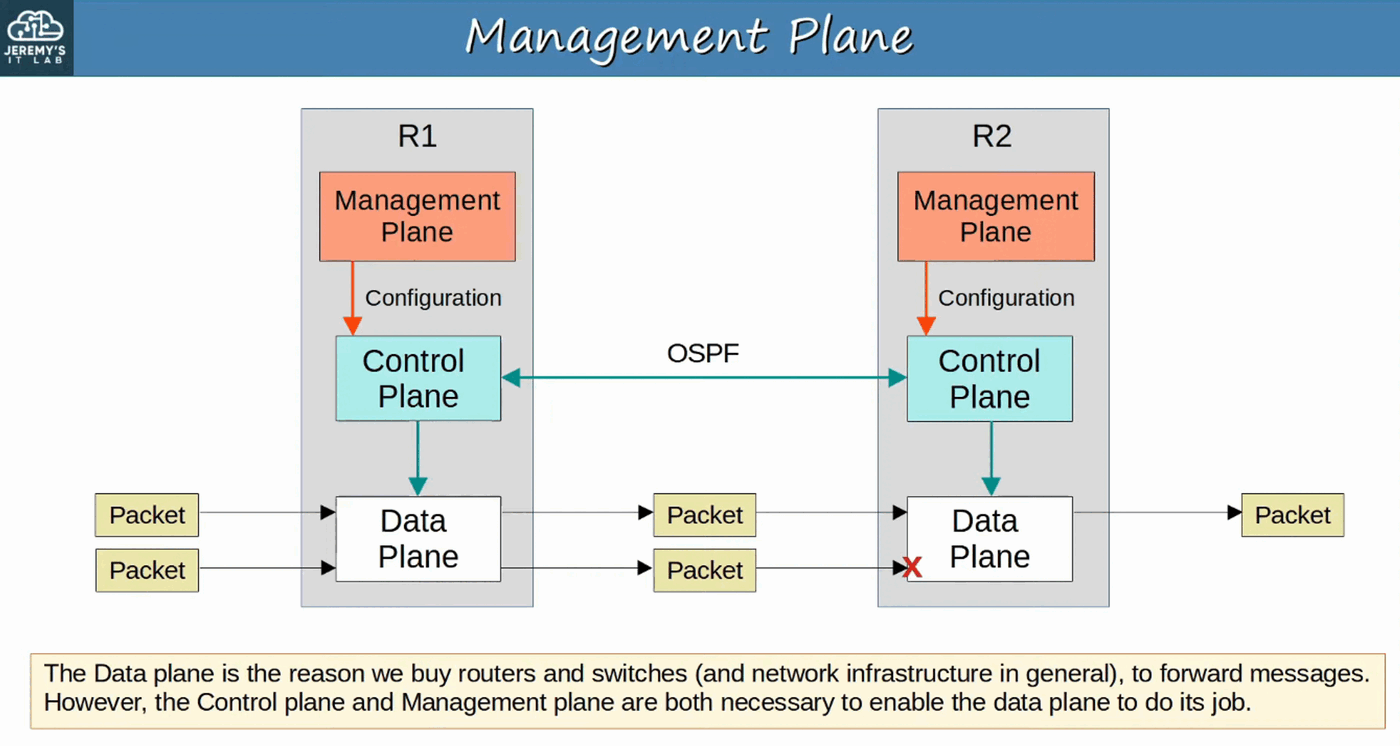
\includegraphics[keepaspectratio,alt={image}]{images/62-introduction-to-network-automation/img-003.png}}
\end{figure}

\section{Software-Defined Networking
(SDN)}\label{software-defined-networking-sdn}

\begin{itemize}
\tightlist
\item
  SOFTWARE-DEFINED NETWORKING (SDN) is an approach to networking that
  centralizes the CONTROL PLANE into an application called a
  \emph{CONTROLLER}
\item
  SDN is also called SOFTWARE-DEFINED-ARCHITECTURE (SDA) or
  CONTROLLER-BASED NETWORKING
\item
  Traditional CONTROL PLANES use a distributed architecture

  \begin{itemize}
  \tightlist
  \item
    For example:

    \begin{itemize}
    \tightlist
    \item
      Each ROUTER in the NETWORK runs OSPF and the ROUTERS share routing
      information and then calculate their preferred routes to each
      destination
    \end{itemize}
  \end{itemize}
\item
  An SDN CONTROLLER centralized CONTROL PLANE functions like calculation
  routes

  \begin{itemize}
  \tightlist
  \item
    That is just an example and how much of the CONTROL PLANE is
    centralized varies greatly
  \end{itemize}
\item
  The CONTROLLER can interact programmatically with the NETWORK DEVICE
  using APIs (Application Programming Interface)
\end{itemize}

\begin{figure}
\centering
\pandocbounded{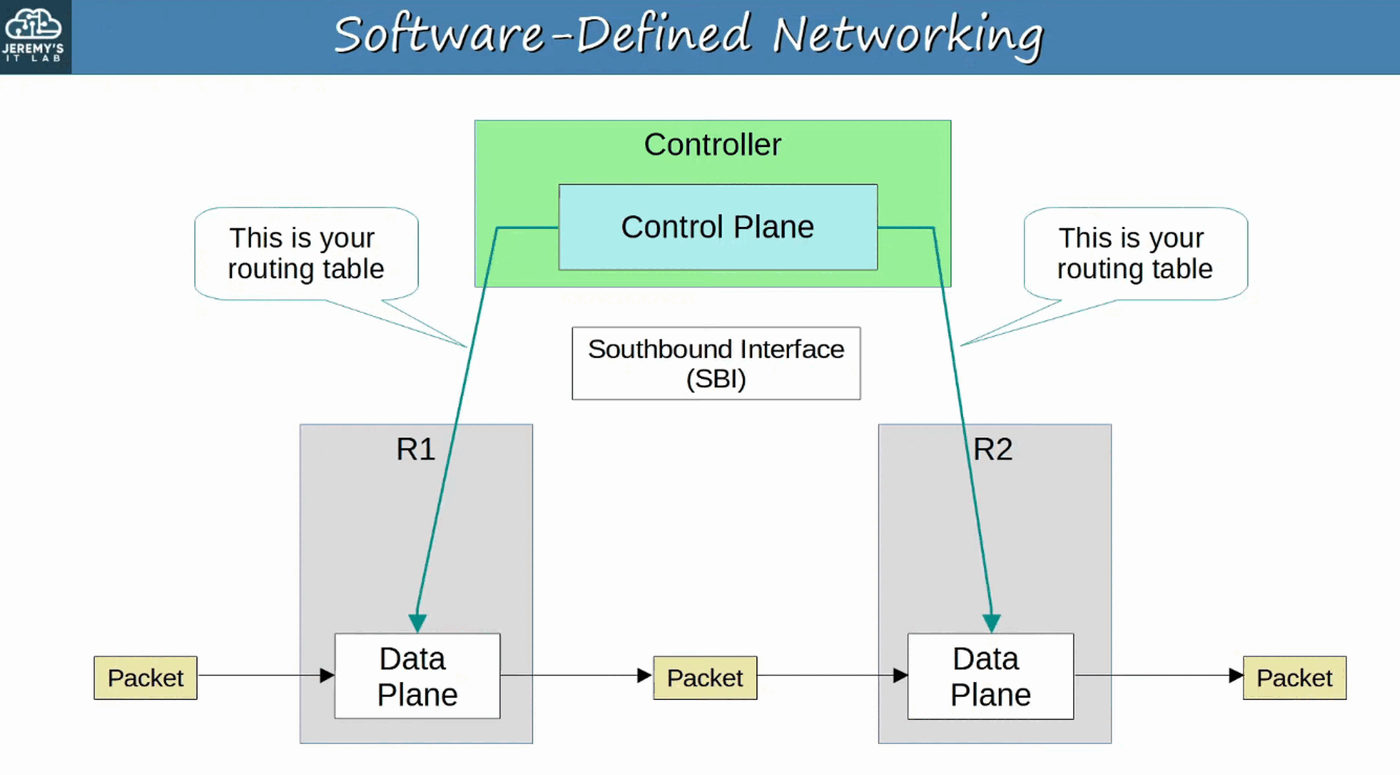
\includegraphics[keepaspectratio,alt={image}]{images/62-introduction-to-network-automation/img-004.png}}
\end{figure}

\section{Southbound Interface (SBI)}\label{southbound-interface-sbi}

\begin{itemize}
\item
  The SBI is used for communications between the CONTROLLER and the
  NETWORK DEVICES it controls
\item
  It typically consists of a COMMUNICATION PROTOCOL and API (Application
  Programming Interface)
\item
  APIs facilitate data exchanges between programs

  \begin{itemize}
  \tightlist
  \item
    DATA is exchanged between the CONTROLLER and the NETWORK DEVICES
  \item
    An API on the NETWORK DEVICES allows the CONTROLLER to access
    information on the DEVICES, control their DATA PLANE TABLES, etc.
  \end{itemize}
\item
  Some examples of SBIs :

  \begin{itemize}
  \tightlist
  \item
    OpenFlow
  \item
    Cisco OpFlex
  \item
    Cisco OnePK (Open Network Environment Platform Kit)
  \item
    NETCONF
  \end{itemize}
\end{itemize}

\section{Northbound Interface (Nbi)}\label{northbound-interface-nbi}

\begin{itemize}
\item
  Using the SBI, the CONTROLLER communicates with the managed DEVICES
  and gathers information about them:

  \begin{itemize}
  \tightlist
  \item
    The DEVICES in the NETWORK
  \item
    The TOPOLOGY (how the DEVICES are connected together)
  \item
    The available INTERFACES on each DEVICE
  \item
    Their CONFIGURATIONS
  \end{itemize}
\item
  The NORTHBOUND INTERFACE (NBI) is what allows us to:

  \begin{itemize}
  \tightlist
  \item
    Interact with the CONTROLLER
  \item
    Access the DATA it gathers about the NETWORK
  \item
    Program the NETWORK
  \item
    Make changes to the NETWORK via the SBI
  \end{itemize}
\item
  A REST API (Representational State Transfer) is used on the controller
  as an interface for APPS to interact with it
\item
  OSGi (Java Open Services Gateway Initiative) - Java based NBI API
\item
  DATA is sent in a structured (\emph{serialized}) format such as JSON
  or XML

  \begin{itemize}
  \tightlist
  \item
    This makes it easier for programs to use the DATA
  \end{itemize}
\end{itemize}

\begin{figure}
\centering
\pandocbounded{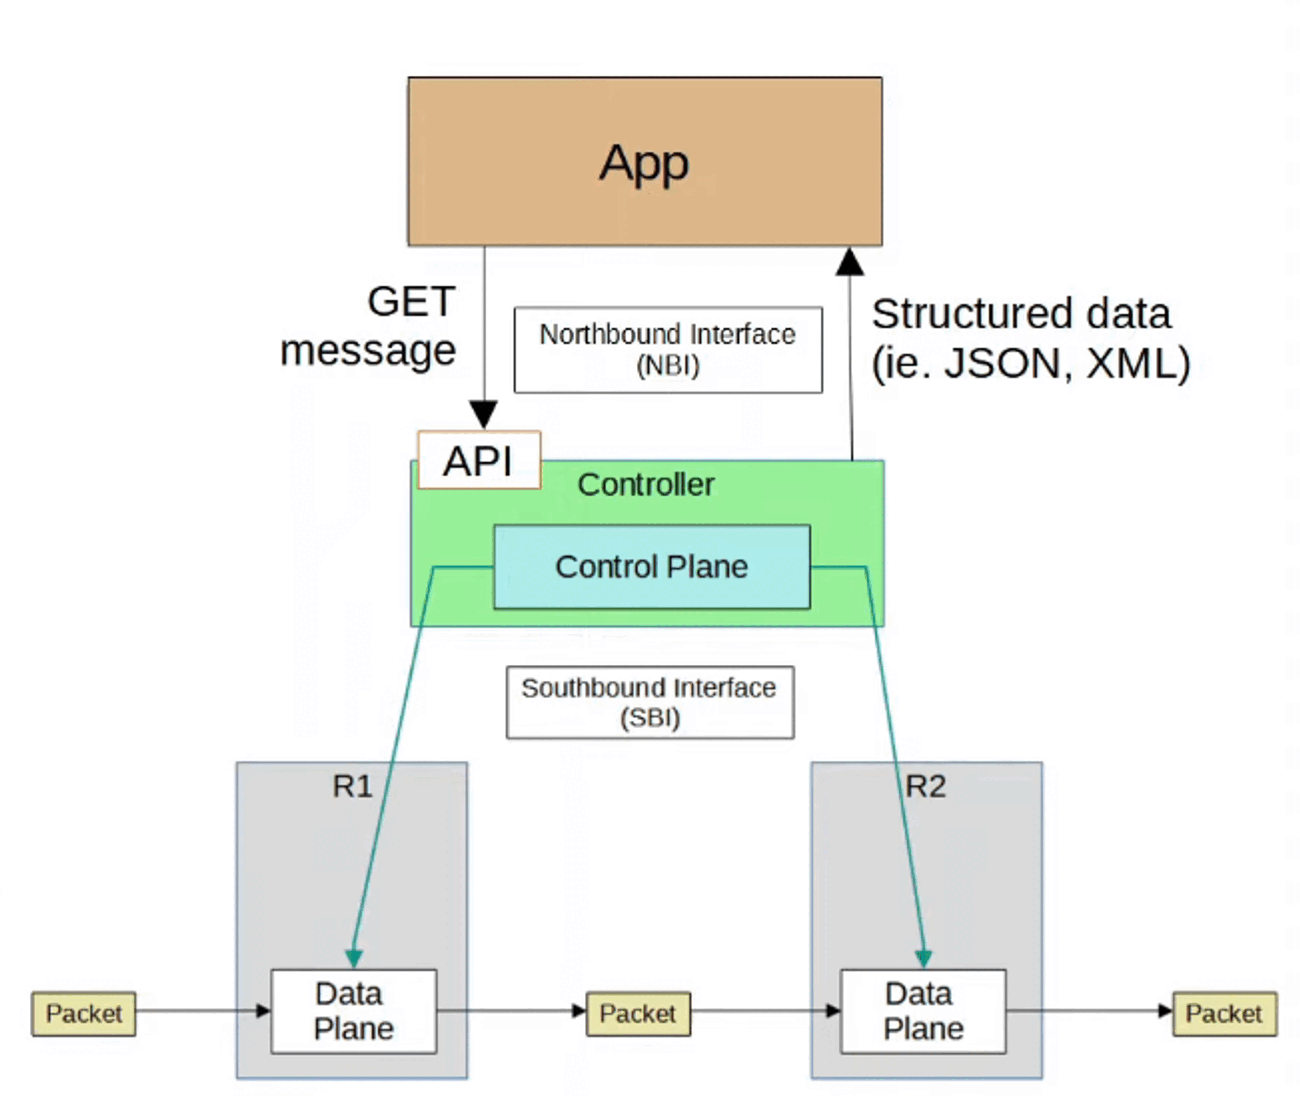
\includegraphics[keepaspectratio,alt={image}]{images/62-introduction-to-network-automation/img-005.png}}
\end{figure}

\section{Automation in Traditional Networks vs
SDN}\label{automation-in-traditional-networks-vs-sdn}

\begin{itemize}
\tightlist
\item
  Networking tasks can be automated in traditional NETWORK architectures
  too:

  \begin{itemize}
  \tightlist
  \item
    SCRIPTS can be written (ie: using Python) to push commands to many
    DEVICES at once
  \item
    Python with good use of REGULAR EXPRESSIONS can parse through
    ``show'' commands to gather information about network devices
  \end{itemize}
\item
  However, the robust and centralized DATA collected by SDN CONTROLLERS
  greatly facilitates these functions

  \begin{itemize}
  \tightlist
  \item
    The CONTROLLER collects information about all DEVICES in the NETWORK
  \item
    NORTHBOUND APIs allow APPS to access information in a format that is
    easy for programs to understand (ie: JSON and XML)
  \item
    The centralized DATA facilitates network-wide analytics
  \end{itemize}
\item
  SDN Tools can provide the benefits of automation without the
  requirement of third-party scripts and apps.

  \begin{itemize}
  \tightlist
  \item
    You don't need expertise in automation to make use of SDN Tools
  \item
    However, APIs allow third-party applications to interact with the
    CONTROLLER, which can be very powerful
  \end{itemize}
\end{itemize}

\begin{quote}
Although SDN and automation aren't the same thing, the SDN architecture
greatly facilitates the automation of various tasks in the network via
the SDN CONTROLLER and APIs
\end{quote}
